% % % % % % % % % % % % % % % % % % % % % % % % % % % % % % % % % % % % % % % % % % % %
%                                                                                     %
% Short Sectioned Assignment LaTeX Template Version 1.0 (5/5/12)                      %
% This template has been downloaded from: http://www.LaTeXTemplates.com               %
%                                                                                     %
% Original author:  Frits Wenneker (http://www.howtotex.com)                          %
%                                                                                     %
% Modified by: Fco Javier Sueza Rodríguez (fcosueza@disroot.org)                      %
%                                                                                     %
% Changes:                                                                            %
%	    - Custom Chapters, Sections and Subsections (titlesec package)                %
%           - Document type scrbook (oneside)                                         %
%           - Use babel-lang-spanish package and marvosym                             %
%           - Use hyperref, enumitem, tcolorbox and glossaries packages               %
%           - Use Time New Roman (mathptmx), Helvetic and Courier fonts               %
%                                                                                     %
% License: CC BY-NC-SA 3.0 (http://creativecommons.org/licenses/by-nc-sa/3.0/)        %
%                                                                                     %
% % % % % % % % % % % % % % % % % % % % % % % % % % % % % % % % % % % % % % % % % % % %

%-----------------------------------------------%
%	              Packages                  %
%-----------------------------------------------%

\documentclass[paper=a4, fontsize=11pt, oneside]{scrbook}

% ---- Text Input/Output ----- %

\usepackage[T1]{fontenc}
\usepackage[utf8]{inputenc}
\usepackage{mathptmx}
\usepackage[scaled=.92]{helvet}
\usepackage{courier}
\usepackage[indent=12pt]{parskip}

\usepackage{geometry}
\geometry{verbose,tmargin=3cm,bmargin=3cm,lmargin=2.6cm,rmargin=2.6cm}

% ---- Language ----- %

\usepackage[spanish]{babel}
\usepackage{marvosym}

% ---- Another packages ---- %

\usepackage{amsmath,amsfonts,amsthm}
\usepackage{graphics,graphicx}
\usepackage{titlesec}
\usepackage{fancyhdr}
\usepackage{tcolorbox}
\usepackage{hyperref}
\usepackage{enumitem}
\usepackage[automake]{glossaries}

%--------------------------------------------------------------------%
%                      Customizing Document                          %
%--------------------------------------------------------------------%


% ----------- Custom Chapters, Sections and Subsections -------------- %

\titleformat{\chapter}[display]
			{\bfseries\Huge}
			{Tema \ \thechapter} {0.5ex}
			{\vspace{1ex}\centering}

\titleformat{\section}[hang]
			{\bfseries\Large}
			{\thesection}{0.5em}{}

\titleformat{\subsection}[hang]
			{\bfseries\large}
			{\thesubsection}{0.5em}{}

\titleformat{\subsubsection}[hang]
			{\bfseries\large}
			{\thesubsubsection}{0.5em}{}

\hypersetup{
    colorlinks=true,
    linkcolor=black,
    urlcolor=magenta
}

% ------------------- Custom heaaders and footers ------------------- %

\pagestyle{fancyplain}

\fancyhead[]{}
\fancyfoot[L]{}
\fancyfoot[C]{}
\fancyfoot[R]{\thepage}

\renewcommand{\headrulewidth}{0pt} % Remove header underlines
\renewcommand{\footrulewidth}{0pt} % Remove footer underlines

\setlength{\headheight}{13.6pt} % Customize the height of the header

% --------- Numbering equations, figures and tables ----------------- %

\numberwithin{equation}{section} % Number equations within sections
\numberwithin{figure}{section} % Number figures within sections
\numberwithin{table}{section} % Number tables within sections

% ------------------------ New Commands ----------------------------- %

\newcommand{\horrule}[1]{\rule{\linewidth}{#1}} % Create horizontal rule command


%----------------------------------------------------------------------------------------
%	TÍTULO Y DATOS DEL ALUMNO
%----------------------------------------------------------------------------------------

\title{
\vspace{10ex}
\normalfont \normalsize
\huge \textbf{Tarea 4: Contenidos Multimedia en la Web (Imagen, Audio y Vídeo)}
}
\author{Francisco Javier Sueza Rodríguez}
\date{\normalsize\today}

%----------------------------------------------------------------------------------------
%                                     DOCUMENTO
%----------------------------------------------------------------------------------------
\begin{document}

\maketitle

\thispagestyle{empty}

\vspace{65ex}

\begin{center}
    \begin{tabular}{l l}
        \textbf{Centro}: & IES Aguadulce \\
        \textbf{Ciclo Formativo}: & Desarrollo Aplicaciones Web (Distancia)\\
        \textbf{Asignatura}: & Diseño de Interfaces Web\\
        \textbf{Tema}: & Tema 4 -  Contenido Multimedia en la Web (Imagen, Audio y Vídeo)\\
    \end{tabular}
\end{center}

\newpage

\tableofcontents

\newpage

\section{Ejercicio 1: Imagen Composición}
En este ejercicio se han descargado varias imágenes para nuestra web y se ha creado una composición con GIMP. En los siguientes apartados, se van a dar respuesta a las diferentes cuestiones que se plantean en el enunciado del ejercicio.

\subsection{Apartado A}
Se ha creado una \textbf{captura de pantalla} del editor VS Code, para usarla como fondo de nuestra composición. A esta imagen se le ha asignado una licencia \textbf{CC Zero}, es decir, es una imagen de dominio público.

Como podemos ver en la \href{https://creativecommons.org/publicdomain/zero/1.0/deed.es}{web de Creative Commons}, esta licencia no tiene ningún tipo de restricción, cediendo todos los derechos de la imagen creada. Se ha decidido emplear esta licencia por es la menos restrictiva y se le quería otorgar a cualquier usuario el máximo de libertad posible para hacer con ella lo que les parezca oportuno.

Cabe destacar que la licencia se ha añadido como metadatos generados en la página de Creative Commons en una archivo XMP, ya que al añadir el logo de la licencia a la composición final si se hubiera añadido a esta imagen también el logo aparecería por duplicado.

\subsection{Apartado B}
El siguiente paso ha sido buscar una imagen relacionada con el \textbf{desarrollo web}, encontrándose una imagen con la palabra \textbf{Web} donde en su interior aparece texto con muchas de las tecnologías relacionadas con el desarrollo web.

La licencia de esta imagen, como podemos ver \href{https://pxhere.com/es/photo/841903}{en la web de descarga}, es también \textbf{CC Zero}, es decir, es una imagen de \textbf{dominio público}.

\subsection{Apartado C}
Se ha escogido, para el nuevo producto ha sido también \textbf{CC Zero}, ya que al igual que con la captura de pantalla, se ha querido dar el mayor grado de libertad a los posibles usuario que quieran usar esta composición.

En la siguiente captura, podemos ver todos los datos de la imagen que nos pide en enunciado.

\begin{figure}[H]
    \centering
    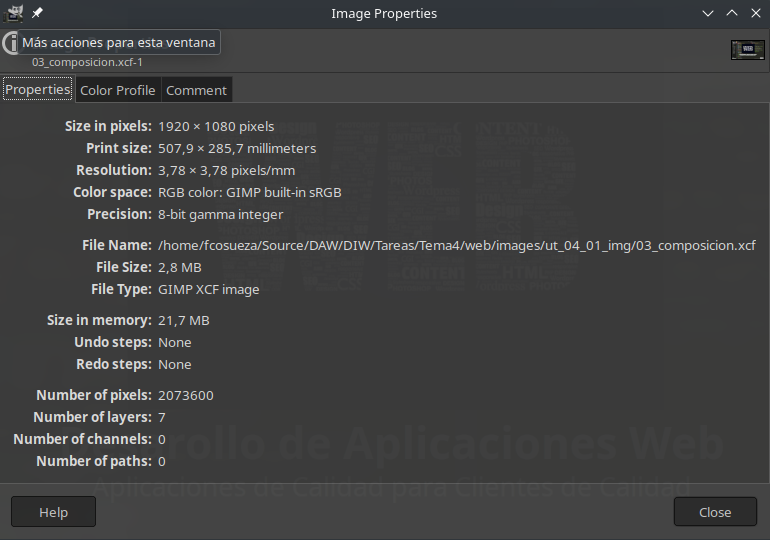
\includegraphics[scale=0.43]{propiedades.png}
\end{figure}

El \textbf{formato} elegido para la composición final ha sido \textbf{WebP}. Se ha elegido este formato porque genera archivos que en relación a su reducido tamaño, tienen más calidad que PNG.

Si bien es cierto que la gran mayoría de navegadores soportan este formato, hay alguno, en concreto Internet Explorer, que no lo soporta aún, como podemos ver en \href{https://caniuse.com/webp}{Can I Use}. Si se tiene mucho interés en dar soporte a este navegador, se podría crear una imagen alternativa y crear una media query para que cargue la imagen en otro formato, pero en general, con este formato tenemos más ventajas que inconvenientes.

\section{Ejercicio 2: Imagen Transformación y Optimización}
En este apartado vamos a realizar alguna transformación en la composición creada y a reducir un poco su tamaño, que ya de pos sí es bastante bajo. Para realizar la reducción de tamaño se ha realizado lo siguiente:

\begin{itemize}
    \item \textbf{Reducción de Tamaño}: la propia reducción de tamaño que se nos ha solicitado en el enunciado ya nos ha servido para reducir su peso considerable, así que esta ha sido la primera medida que se ha tomado.
    \item \textbf{Bajara la Calidad}: la segunda medido ha sido bajar la calidad de la imagen cuando la hemos exportado, tanto de la imagen como del canal Alpha, eso ha supuesto también una reducción del peso de la imagen. Tanto esta media como la anterior se han realizado con GIMP.
\end{itemize}

\section{Ejercicio 3: Audio}




% Bibliography

%\newpage
%\bibliography{citas}
%\bibliographystyle{unsrt}

\end{document}